\documentclass[tikz,border=10pt]{standalone}
\usetikzlibrary{shapes.geometric, arrows.meta, positioning}

% Define styles globally
\tikzset{
    decision/.style={diamond, aspect=2, draw, fill=blue!20, text width=5em, text centered, inner sep=0pt},
    block/.style={rectangle, draw, fill=blue!20, text width=5em, text centered, rounded corners},
    line/.style={draw, -Latex},
    every node/.style={font=\sffamily}
}

\begin{document}
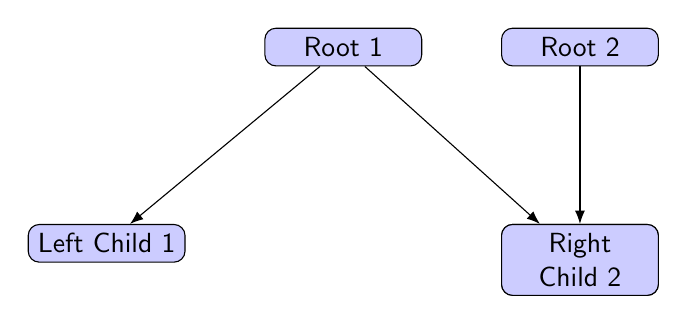
\begin{tikzpicture}[node distance=2cm and 1cm]

    % First tree
    \node [block] (root1) {Root 1};
    \node [block, below left=of root1] (leftChild1) {Left Child 1};
    \node [block, below right=of root1] (rightChild1) {Right Child 1};
    \draw [line] (root1) -- (leftChild1);
    \draw [line] (root1) -- (rightChild1);

    % Second tree
    \node [block, right=of root1] (root2) {Root 2};
    \node [block, below=of root2] (rightChild2) {Right Child 2};
    \draw [line] (root2) -- (rightChild2);

\end{tikzpicture}
\end{document}